\section{Vektorer og vektorfunktioner}

\emph{Forklar om vektorer og vektorfunktioner, herunder hvordan de differentieres.}

En vektor er en pil, der har en retning og en vektor.

Når vi regner med vektorer, så anvender vi kartesisk notation.

Nemt at lave vektorer mellem punkter, da kartesisk notation præcis er $\Delta x$ og $\Delta y$.

Skalering af vektor ved at gange med konstant på begge koordinater.

Enhedscirklen sinus og cosinus, hvordan defineres de

Vektorfunktioner, giver en vektor til et punkt på grafen, ikke injektive nødvendigvis

Den afledte sker ved differentiering af hver koordinatfunktion,
som giver hastighedsvektoren,
dvs. hvilken retning funktionen bevæger sig i, når vi bevæger os langs $t$

\subsection{Bevis af cirklens parameterfremstilling}

\begin{proofw}
    \begin{figure}[h]
        \centering
        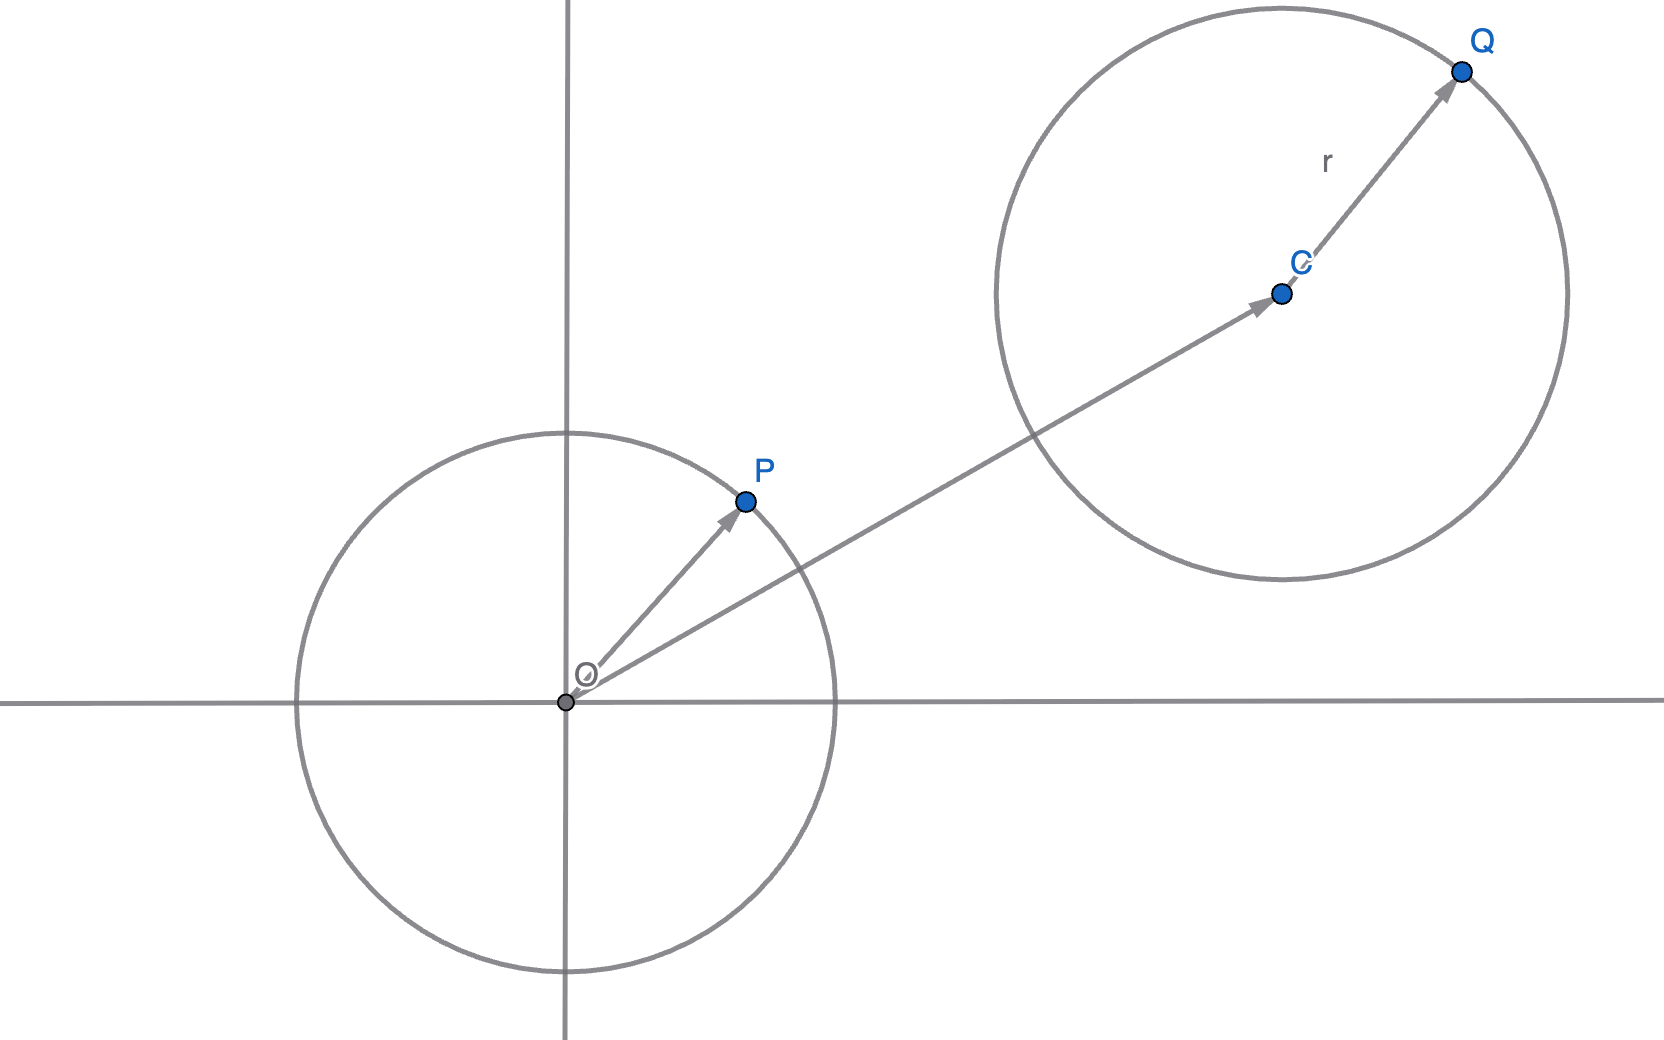
\includegraphics[scale=0.3]{skitser/cirkel.png}
    \end{figure}

    Betragt ovenstående figur, først tager vi tilfældet,
    hvor cirklen har centrum i origo. Her vil alle punkter
    på cirkelperifirien kunne beskrives som en skalering af enhedscirklen, derfor:

    $$
        \vec{OP}=\begin{pmatrix}
            r\cdot \cos(t)
            \\
            r\cdot \sin(t)
        \end{pmatrix}
    $$
    
    For cirklen, der ikke har centrum i origo, er situationen en smule anderledes,
    men vektoren $\vec{CQ}=\vec{OP}$, da cirklerne har samme radius $r$.
    Vi anvender indskudsreglen til at finde:

    $$
        \vec{OQ}=\vec{OC}+\vec{CQ}
    $$

    Disse værdier kender vi, så parameterfremstillingen bliver:

    $$
    \begin{pmatrix}
        x \\ y
    \end{pmatrix}
    =\begin{pmatrix}
        a \\ b
    \end{pmatrix}
    +
    \begin{pmatrix}
        r \cdot \cos(t)
        \\
        r \cdot \sin(t)
    \end{pmatrix}
    =\begin{pmatrix}
        a+ r \cdot \cos(t)
        \\
        b+ r \cdot \sin(t)
    \end{pmatrix}
    $$

\end{proofw}
